% !TEX root = paper.tex

\section {Results}
\label{sec:results}
\subsection{$p_{\mathrm{T}}$ and multiplicity dependence}

\begin{figure}[h!]
		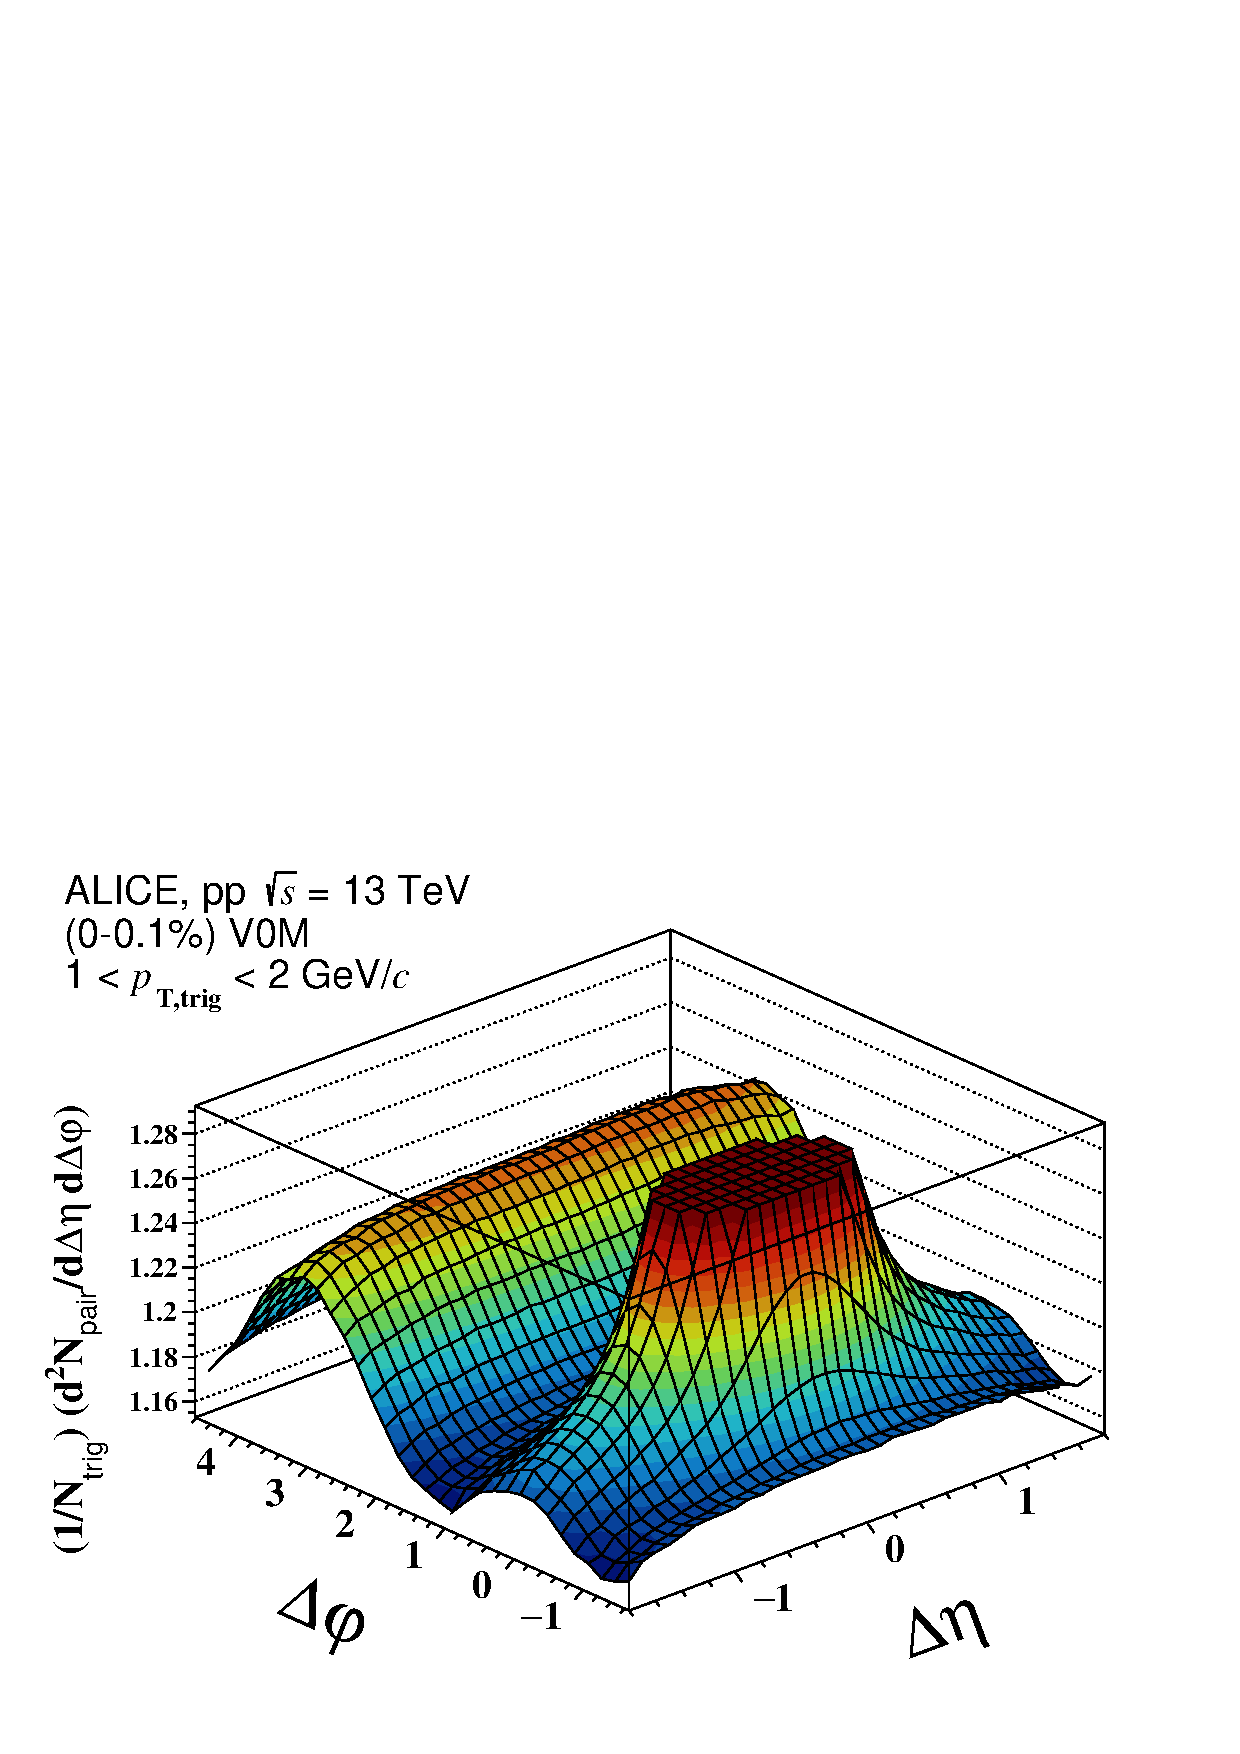
\includegraphics[width=0.3 \textwidth]{figures/CorrForAN_C_0_0_0_11.pdf} 
		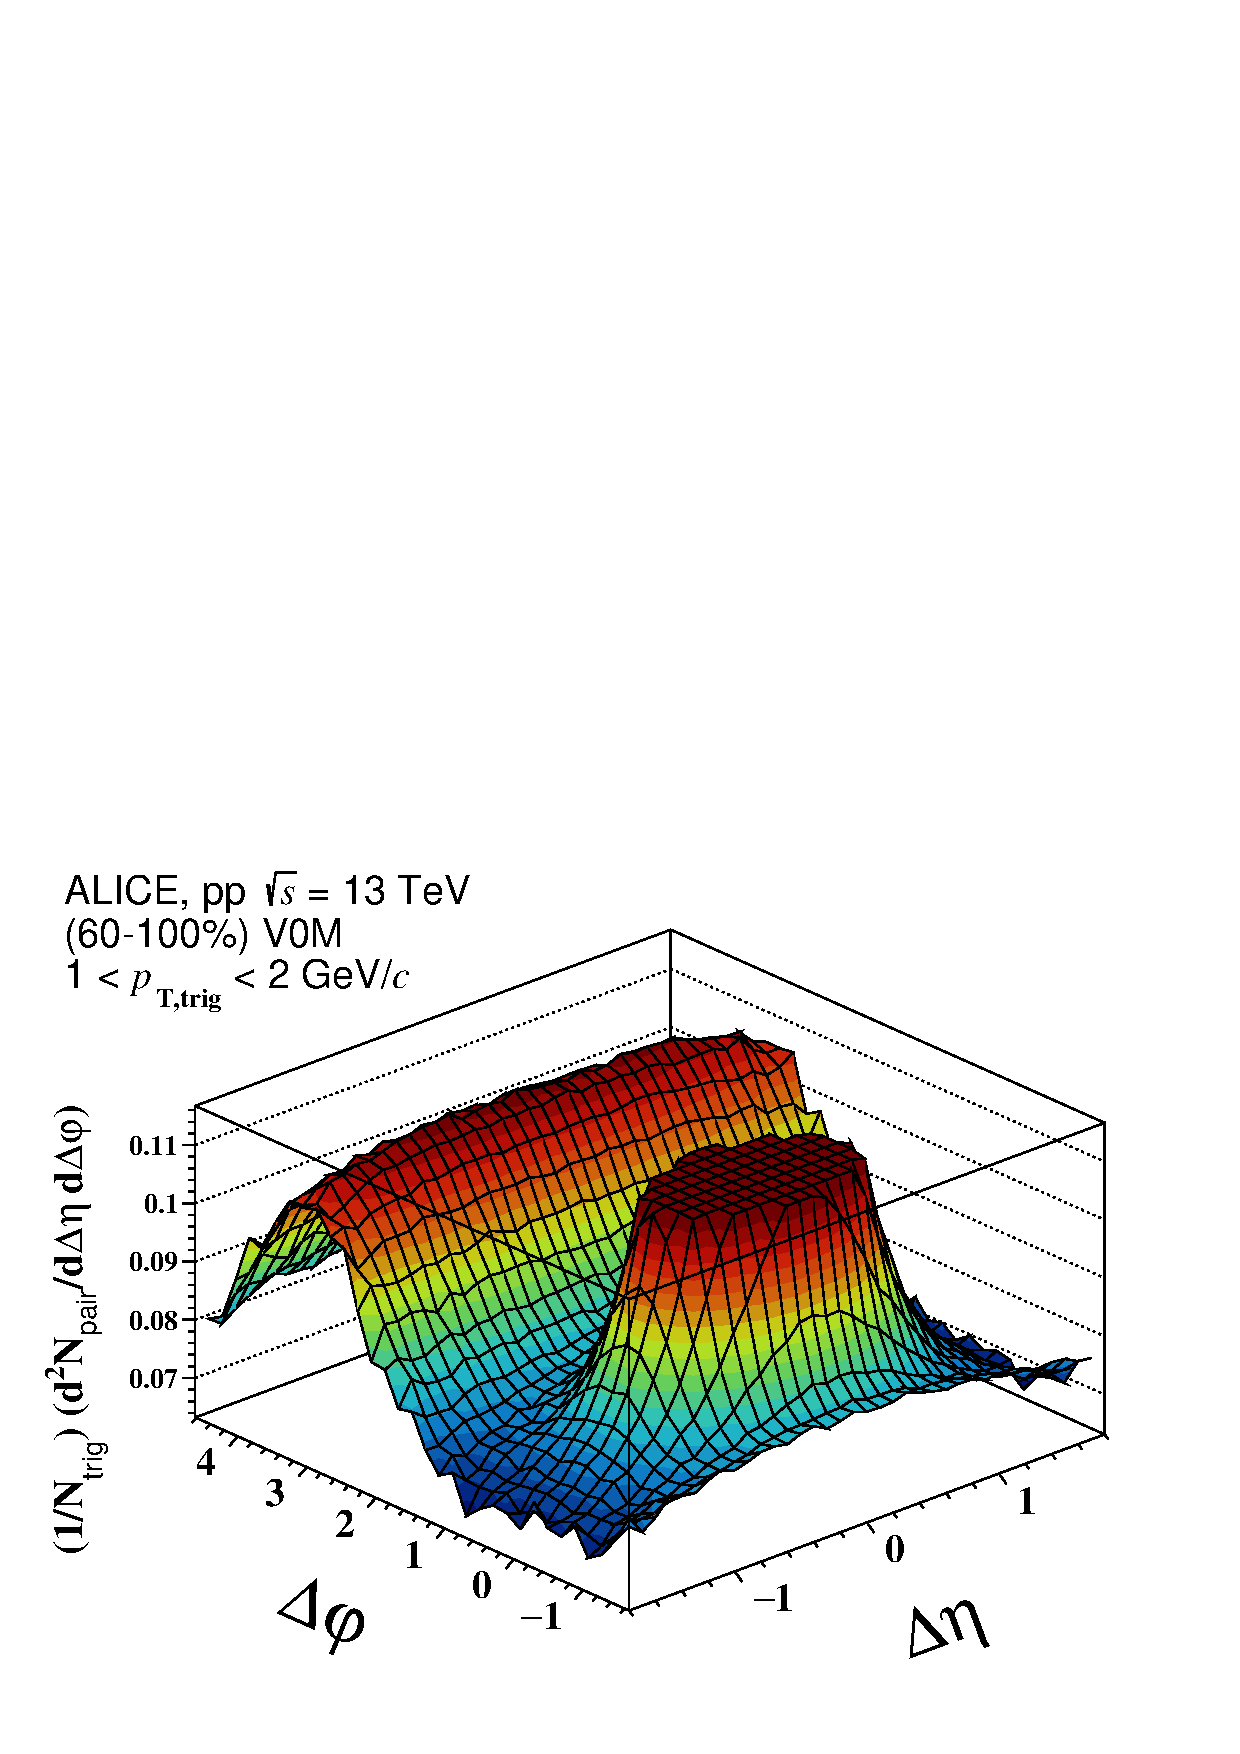
\includegraphics[width=0.3 \textwidth]{figures/CorrForAN_C_0_0_4_11.pdf} 
		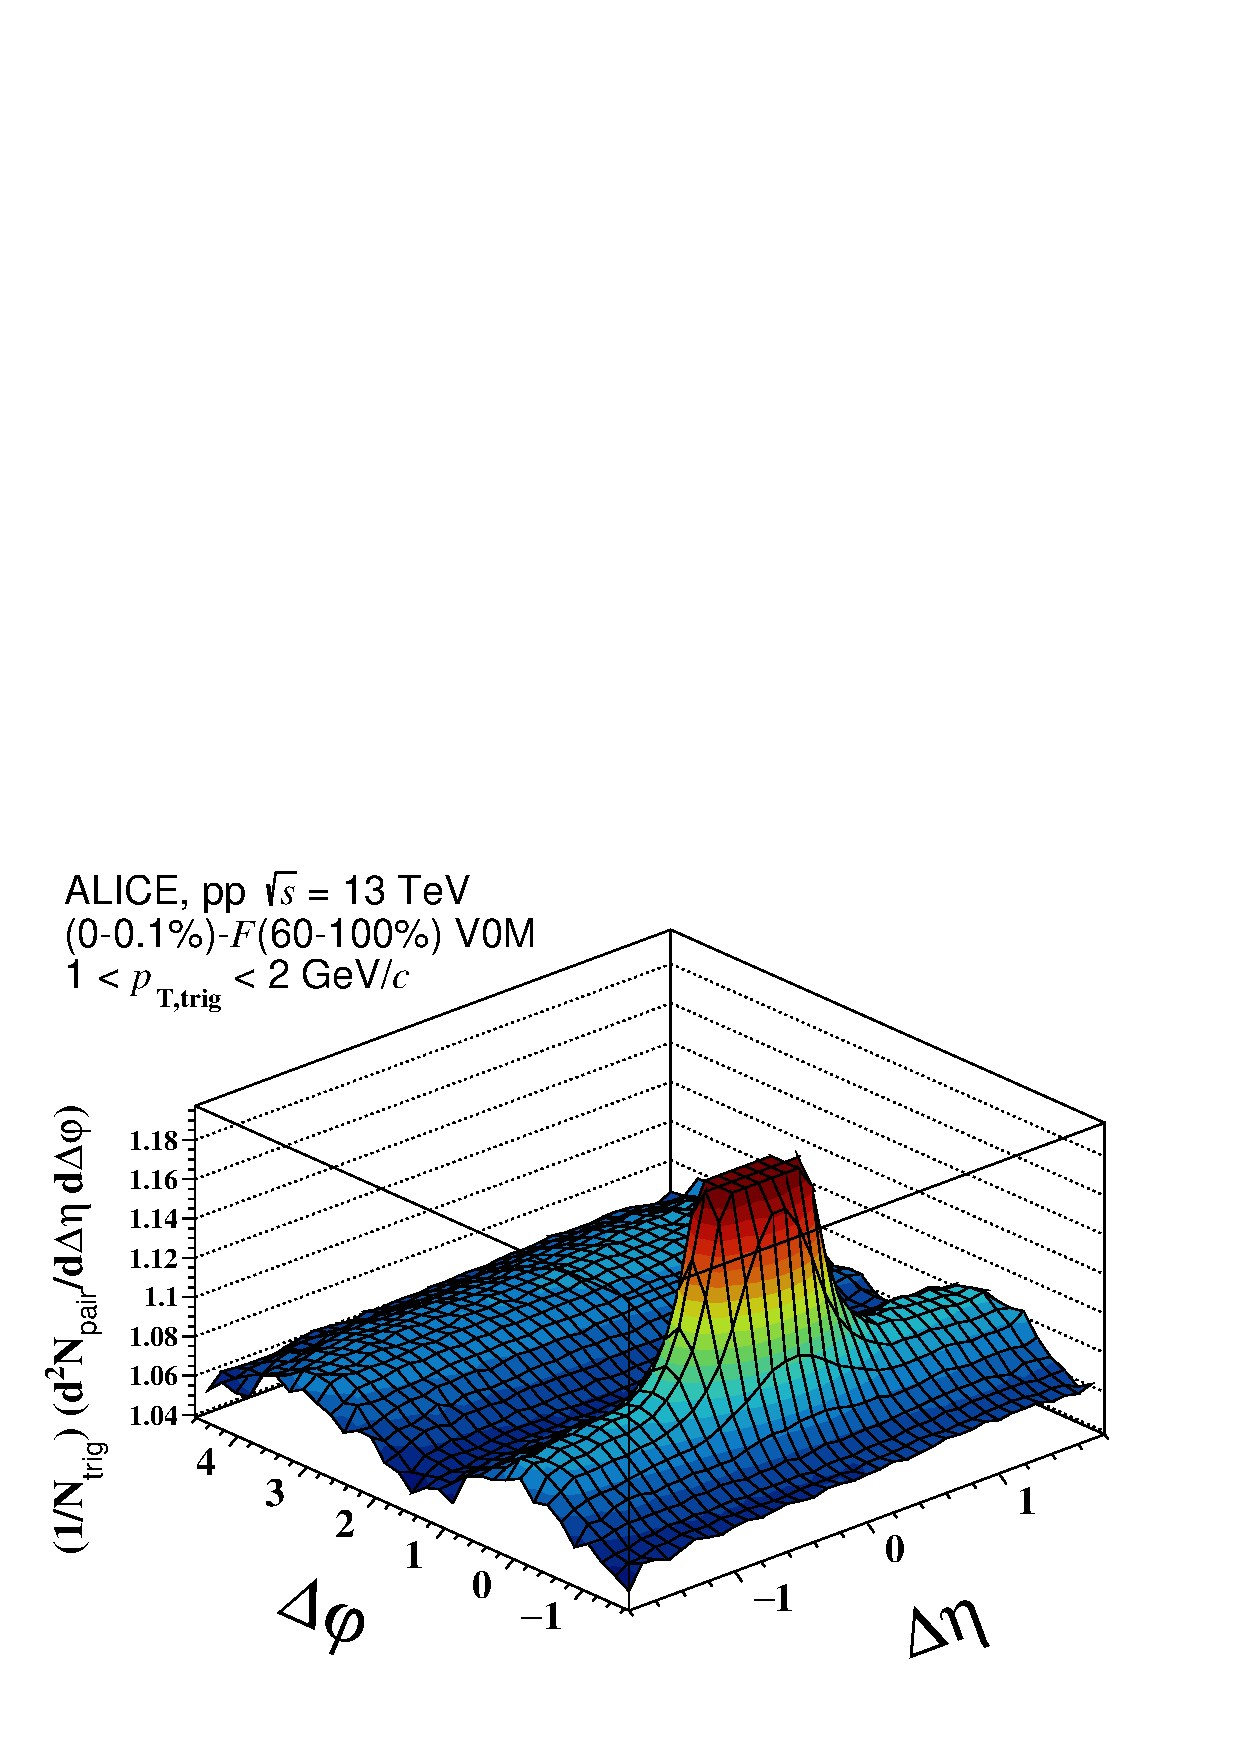
\includegraphics[width=0.3 \textwidth]{figures/CorrForAN_C_SUB_0_0_0_11.pdf} 
\caption{Two-particle correlation functions as functions of $\Delta\eta$ and $\Delta\varphi$ for HM(0--0.1\%, left) and LM(60--100\%, middle) events in $\sqrt{s}=13$ pp collisions. The subtracted one as (0--0.1)\%-$F$(60--100\%) is shown on the right. Note that the near-side jet peaks exceed the chosen range of the $z$-axis. The intervals of $\pttrig$ and $\ptassoc$ are 1~$<\it{p}_{\rm{T}}<$~2~GeV/$c$ in all cases.}
\label{fig:doubleridge}
\end{figure}
\begin{figure}[h!]
			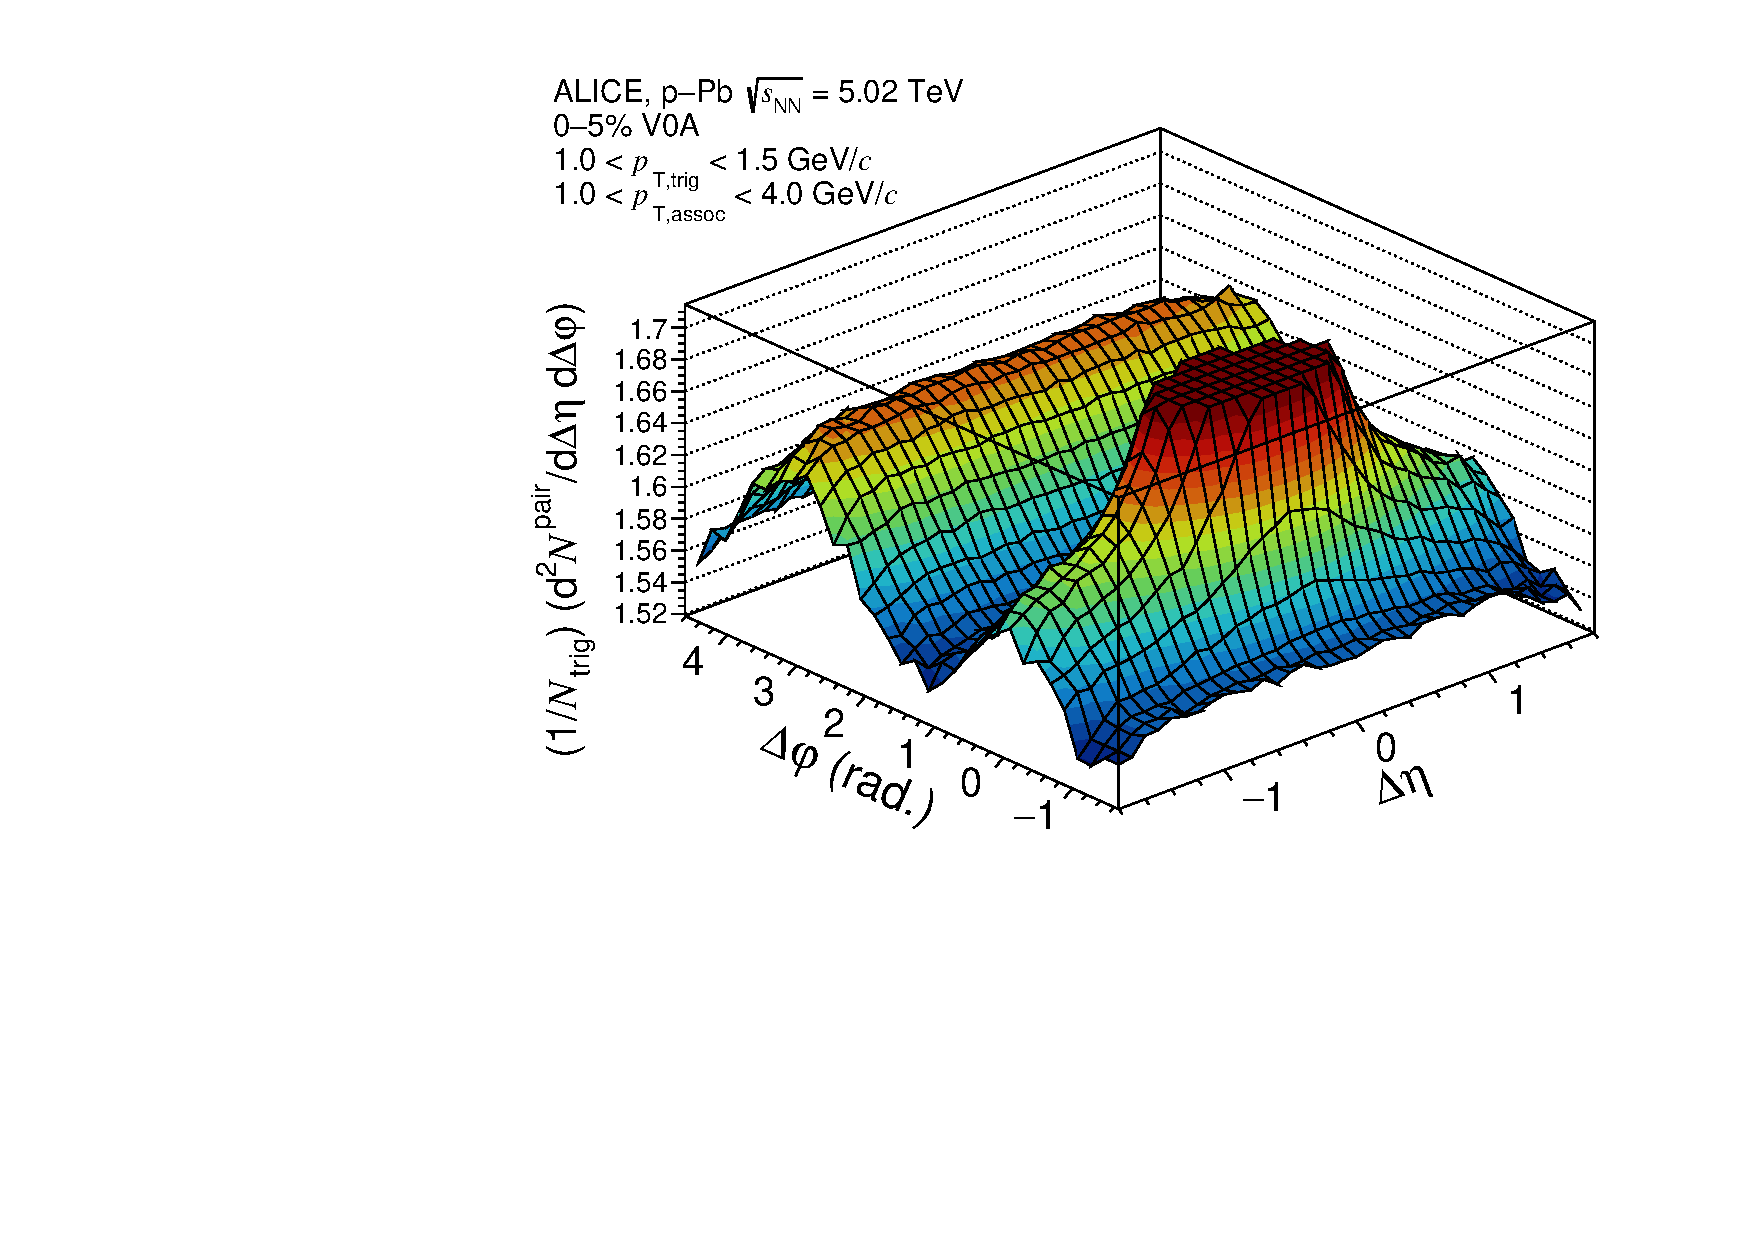
\includegraphics[width=0.3 \textwidth]{figures/corr_1_0_6.pdf}
			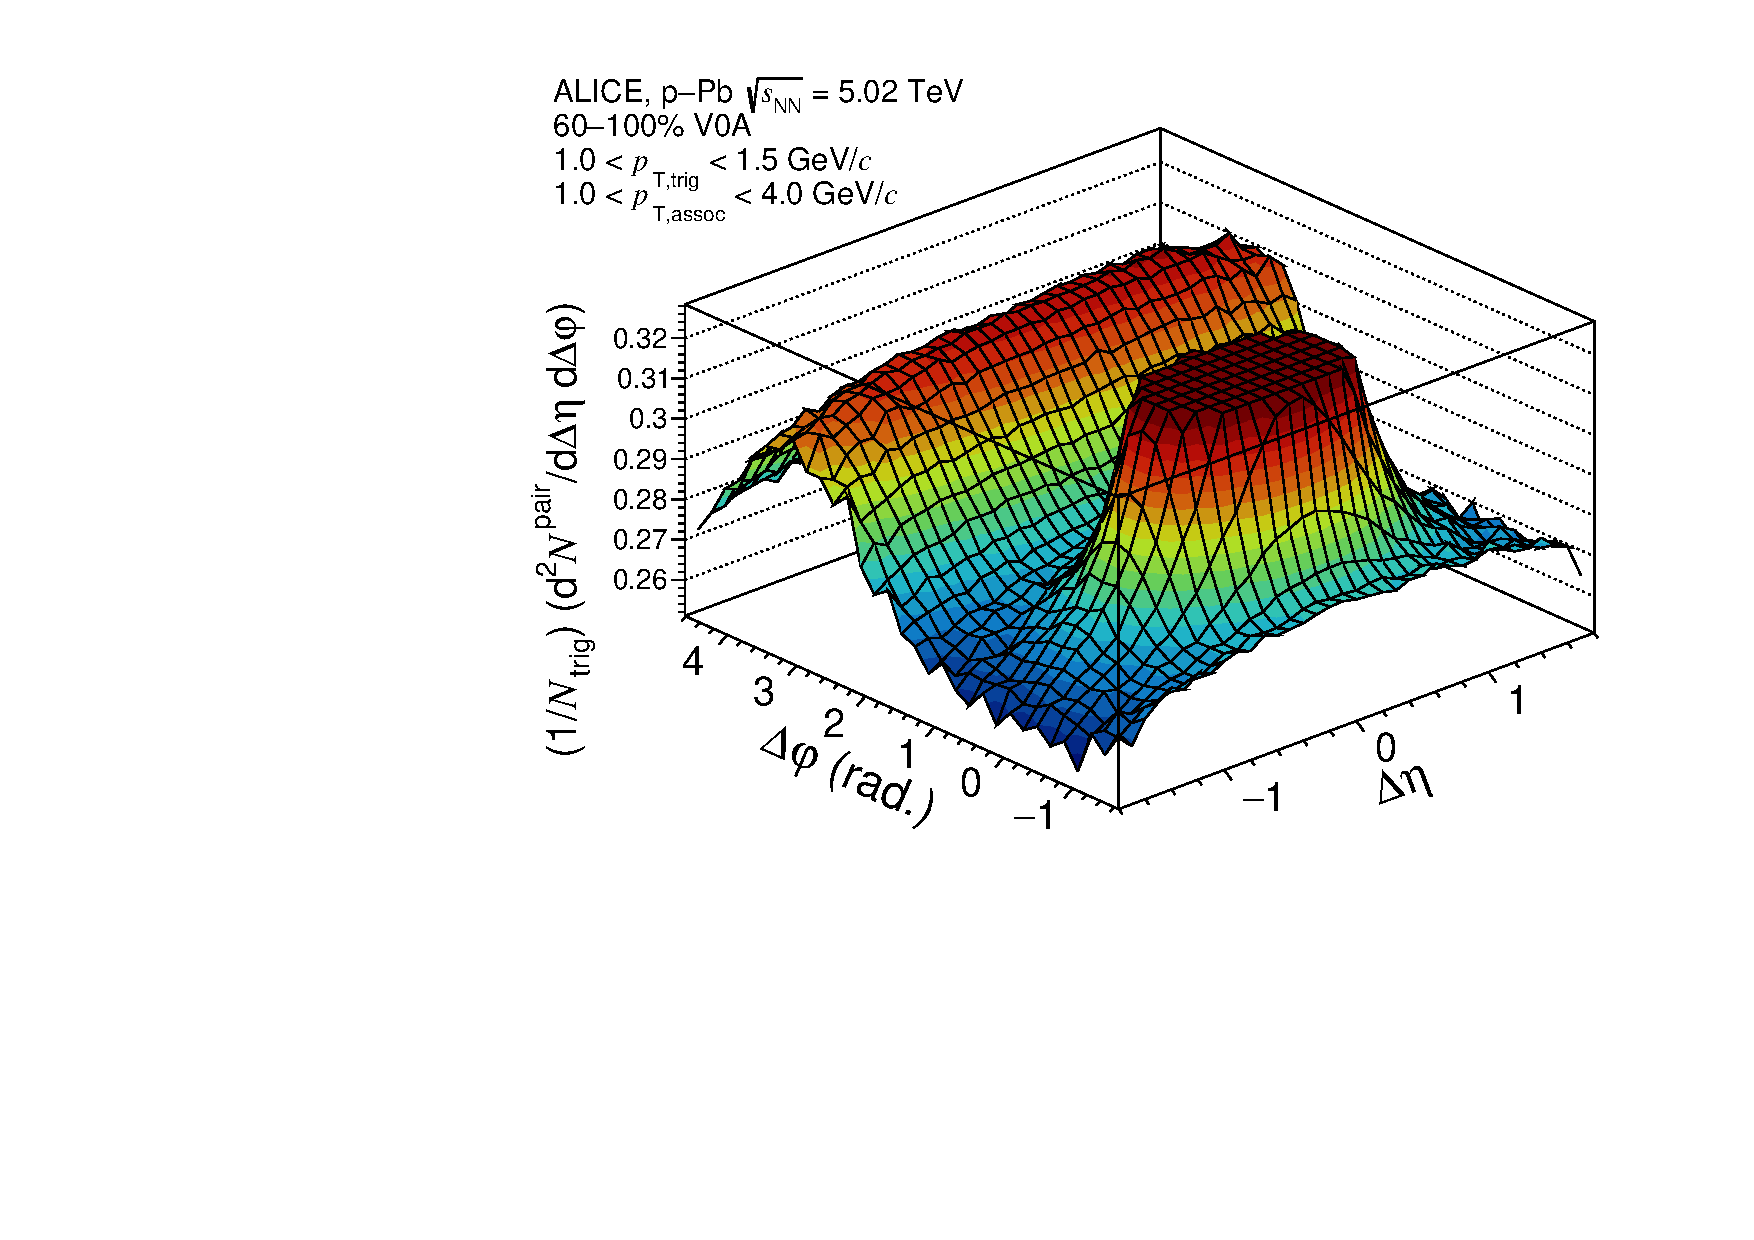
\includegraphics[width=0.3 \textwidth]{figures/corr_1_5_6.pdf}
			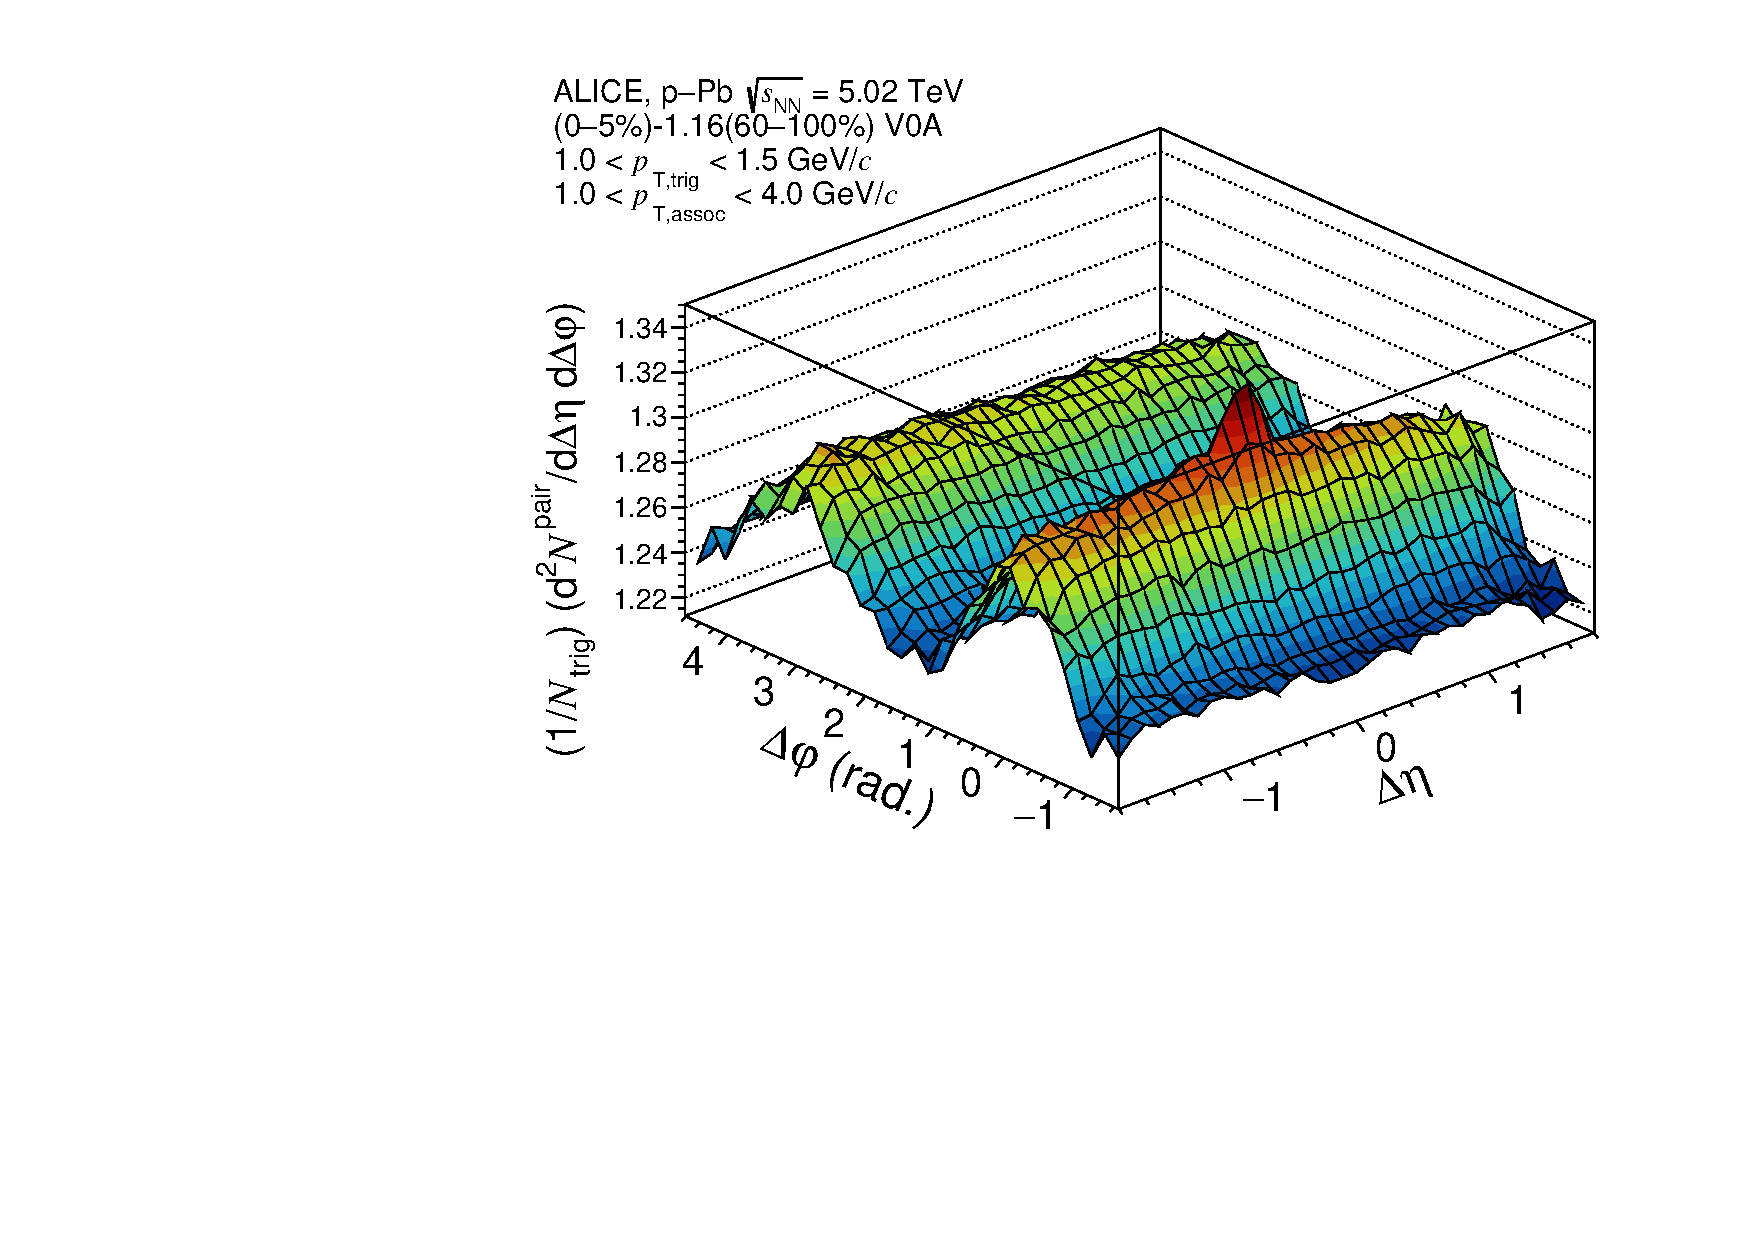
\includegraphics[width=0.3 \textwidth]{figures/corr_sub_temp_1_0_6.pdf}
\caption{Two-particle correlation functions as functions of $\Delta\eta$ and $\Delta\varphi$ for HM(0--5\%, left) and LM(60--100\%, middle) events in $\sqrt{s_{\mathrm{NN}}}=5.02$ TeV p-Pb collisions. The subtracted one as (0--5)\%-$F$(60--100\%) is shown on the right. Note that the near-side jet peaks exceed the chosen range of the $z$-axis. The intervals of $\pttrig$ and $\ptassoc$ are 1~$<\it{p}_{\rm{T}}<$~2~GeV/$c$ in all cases.}
\label{fig:doubleridgepPb}
\end{figure}

Two-dimensional correlation distributions in $\sqrt{s}=13$ TeV pp collisions are shown in Fig.~\ref{fig:doubleridge} for the high-multiplicity (0--0.1\%, left), low-multiplicity (60--90\%, middle), and the subtracted one as (0--5)\%-$F$(60--100\%) on the right. Similarly, the ones in $\sqrt{s_{\mathrm{NN}}}=5.02$ TeV p-Pb collisions are shown in Fig.~\ref{fig:doubleridgepPb}. The $F$ values can be found in Tab.~\ref{tab:Fpp} and \ref{tab:FpPb}, which come from the LM-template fit in a given multiplicity percentile as described in Sec.~\ref{sec:ana}. 
The $z$-axes for the yield of the correlations is properly scaled in order to zoom in the larger $\Delta\eta$ region, as a result, the jet peaks are sheared off in both figures. The flow modulations structure is clearly observed in the HM class while it is not seen in the LM-template. The away-side regions are populated mostly by back-to-back jet correlations for the HM and LM events but they are reduced and comparable to the one in near-side in $\Delta\eta > 1.6$. The jet peak in near-side region is remaining on the LM subtracted ones and the LM-template fit uses only $1.6< \Delta\eta < 1.8$.

\begin{figure}[h!]
	\centering
	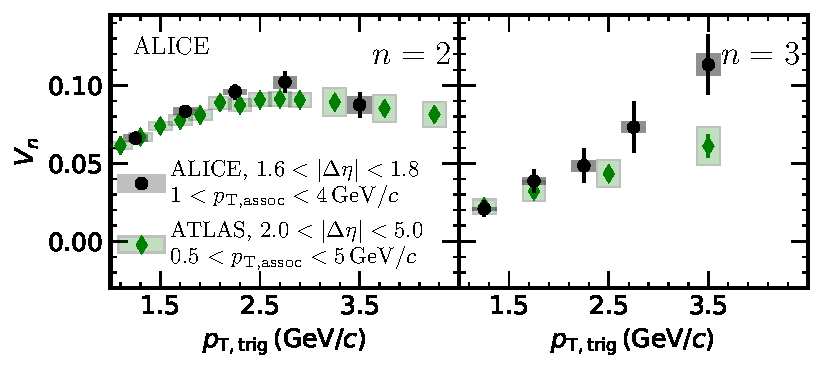
\includegraphics[width=0.9 \textwidth]{figures/Fig2_vn.pdf} 
	\caption{The magnitude of $v_2$ (left) and $v_3$ (right) as a function of $p_\mathrm{T}$. The results are compared to ATLAS measurements~\cite{Aaboud:2016yar}. Note that the event multiplicity definition, $p_{\mathrm{T},assoc}$ range, and $|\Delta\eta|$ acceptance are different.}
	\label{fig:vn}
\end{figure}

The extracted $v_2$ and $v_3$ are shown as a function of $p_{\mathrm{T},trig}$ (GeV/c) in Fig.~\ref{fig:vn}. These results are obtained from the $\sqrt{s}=13$ TeV pp LM-template fits for the high multiplicity percentile of $0-0.1\%$. The results are compared to ATLAS results in~\cite{Aaboud:2016yar} where the same method was used to extract $v_2$ and $v_3$. It should be noted that the $\Delta\eta$ and $p_{\mathrm{T},assoc}$ ranges are larger in the ATLAS results at $2.0<|\Delta\eta|<5.0$ and $0.5<p_{\mathrm{T},assoc}<5$ GeV/c, respectively. 



\begin{figure}[h!]
	\centering
	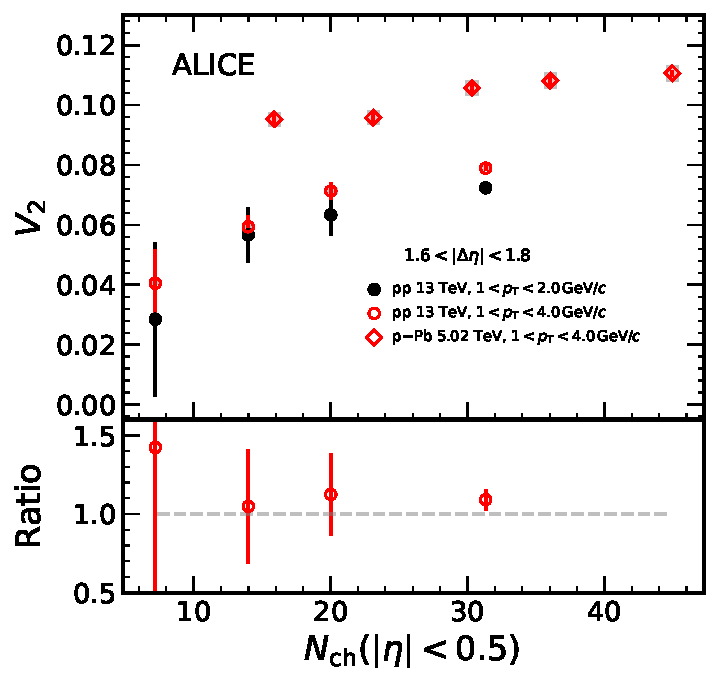
\includegraphics[width=0.6 \textwidth]{figures/Fig6_v2Mult_allSystemsComp2.pdf} 
	\caption{The $v_2$ magnitude for two different collision systems, pp and p-Pb, as a function of multiplicity in the mid-rapidity. Additionally, two different $p_\mathrm{T}$ bins, $1.0<p_\mathrm{T}<2.0$ GeV/c and $1.0<p_\mathrm{T}<4.0$ GeV/c, are presented for pp collisions. The systems are differentiated with two different markers, circles and rhombuses, for pp and p-Pb respectively. The $p_\mathrm{T}$ bins, are differentiated with different colored markers; black for the $1.0<p_\mathrm{T}<2.0$ GeV/c bin and red for the $1.0<p_\mathrm{T}<4.0$ GeV/c bin. In the bottom panel, the ratio $1.0<p_\mathrm{T}<4.0$ bin over the $1.0<p_\mathrm{T}<2.0$ GeV/c bin is presented for pp-collisions and the statistical and systematic errors are combined in quadrature.} 
	\label{fig:v2mult}
\end{figure}

In Fig.\ref{fig:v2mult} the magnitude of $v_2$ as a function of multiplicity is presented for both pp and p-Pb collisions, at $\sqrt{s}=13$ and $\sqrt{s_{NN}}=5.02$ TeV respectively. As in Fig.~\ref{fig:vn}, the large $\Delta\eta$ range is at $1.6<|\Delta\eta|<1.8$ and the associated particle $p_{\mathrm{T},assoc}$ acceptance is $1<p_{\mathrm{T},assoc}<4$ GeV/c for both collision systems. Additionally, pp collisions at 13 TeV with an associated particle $p_{\mathrm{T},assoc}$ acceptance of $1<p_{\mathrm{T},assoc}<2$ GeV/c is presented. The magnitude of $v_2$ is larger in p-Pb collisions, which was observed in Refs.~\cite{ATLAS:2015hzw,ATLAS:2016yzd, Khachatryan:2015lva}. For the two different $p_\mathrm{T}$ bins presented for the pp collisions, the $v_2$ for the $1.0<p_\mathrm{T}<4.0$ GeV/c bin is larger than $v_2$ for the $1.0<p_\mathrm{T}<2.0$ GeV/c bin. This agrees with what is observed in Fig.~\ref{fig:vn}, where the $v_2$ magnitude has its largest value between $2.5<\p_{\mathrm{T,trig}}<3.0$ GeV/c which is above the smaller $p_\mathrm{T}$ bin. The ratio in the bottom panel of Fig.~\ref{fig:v2mult} between the two $p_\mathrm{T}$ bins quantifies an increase of $1\%$ of the larger$p_\mathrm{T}$ bin.
%comparison to ATLAS??
%

\subsection{Event-scale dependence}
\begin{figure}[h!]
	\centering
	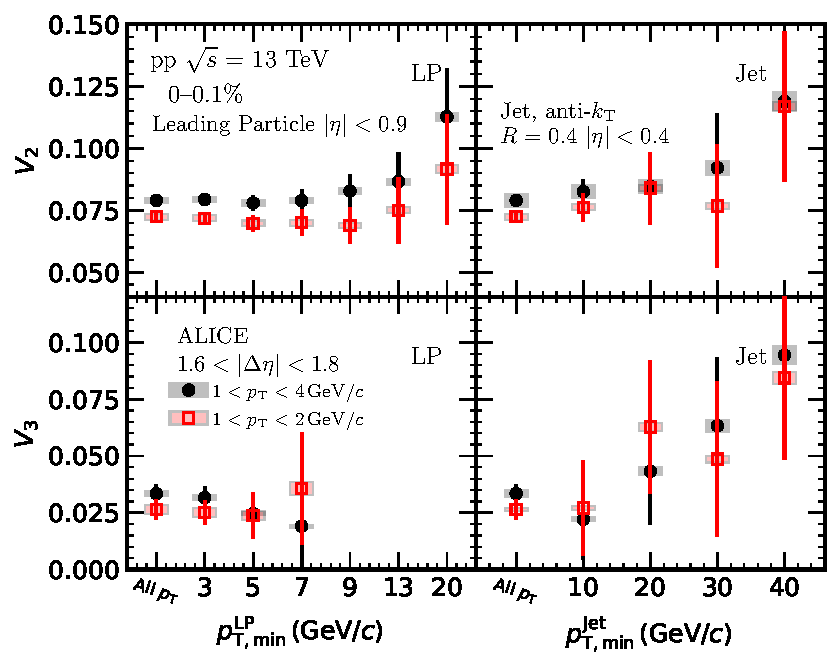
\includegraphics[width=0.6 \textwidth]{figures/Fig4_vn_LP.pdf}
	\caption{The magnitude of $v_2$ (top) and $v_3$ (bottom) as a function of minimum $p_{\mathrm{T}}$ for leading particle (left) and jet (right).}
	\label{fig:LPjet23}
\end{figure}    

Figure~\ref{fig:LPjet23} presents the extracted magnitude of $v_2$ and $v_3$ as function of the minimum $\ptlead$ ($\it{p}^{\rm{LP}}_{\rm{T,min}}$) and $\ptjet$ ($\it{p}^{\rm{jet}}_{\rm{T,min}}$) selections. Both event scale results are obtained from pp collisions at 13 TeV for the multiplicity class of $0-0.1\%$. In these results the leading particle is required to be within $|\eta|<0.9$ and the jets are reconstructed using the anti$-k_\mathrm{T}$ algorithm with R=0.4 and are required to be within $|\eta|<0.4$. Both $v_2$ and$v_3$ show weakly increasing or consistent trend with increasing event-scale selection, with a larger increase of $v_n$ magnitude for the event selection of jets. 